\documentclass[12pt, onecolumn]{IEEEtran}

\usepackage{cite}
% \usepackage[noend]{algpseudocode}
\usepackage{graphicx}
\graphicspath{ {./images/} }
\usepackage{amsmath,amsthm,amssymb,amsfonts}
\usepackage{mathtools}
\usepackage[dvipsnames]{xcolor}
\usepackage{dcolumn}
\usepackage[utf8]{inputenc}
\usepackage{soul}
\usepackage{array}
\usepackage{tabulary}
%---------------------------------------------------------------%
\newtheorem{definition}{Definition}   % 
\theoremstyle{definition}             % alter theorem style: <definition>
\newtheorem{program}{Program}         % [program]
\newtheorem{assumption}{Assumption}   % [assumption]
\newtheorem{example}{Example}         % [example]
\newtheorem{Algorithm}{Algorithm}     % [algorithm]
\newtheorem{policy}{Policy}           % [policy]
\newtheorem{problem}{Problem}         % [problem]
\theoremstyle{remark}                 % alter theorem style: <remark>
\newtheorem{remark}{Remark}           % [remark]
\theoremstyle{plain}                  % alter theorem style: <plain>
\newtheorem{theorem}{Theorem}         % [theorem]
\newtheorem{lemma}{Lemma}             % [lemma]
\newtheorem{corollary}{Corollary}     % [corollary]
%---------------------------------------------------------------%
\newcommand{\eq}{=}
\newcommand{\domZ}{\mathbb{Z}_{*}}
\newcommand{\domP}{\mathbb{Z}_{*}}
\newcommand{\vecOne}{\mathbf{1}}
\newcommand{\ind}{\mathbf{I}}
\newcommand{\mat}{\mathbf}
\newcommand{\Poisson}{\text{Poisson}}
\newcommand{\Bernoulli}{\text{Bernoulli}}
\newcommand{\define}{\triangleq}
\newcommand{\leadto}{\Rightarrow}
\newcommand{\vecG}{\boldsymbol}
\renewcommand{\vec}{\mathbf}
\DeclarePairedDelimiter{\set}{\{}{\}}
\DeclarePairedDelimiter{\norm}{|}{|}
\DeclarePairedDelimiter{\Inorm}{\|}{\|_1}
\DeclarePairedDelimiter{\Paren}{\bigg(}{\bigg)}
\DeclarePairedDelimiter{\Bracket}{\bigg[}{\bigg]}
\DeclarePairedDelimiter{\Brace}{\bigg\{}{\bigg\}}
%
\newcommand{\spaceblank}{\vskip 4mm}
\renewcommand{\baselinestretch}{1.4}
%---------------------------------------------------------------%
\newcommand{\AP}{\dagger}
\newcommand{\ES}{\ddagger}
\newcommand{\apSet}{\mathcal{K}}
\newcommand{\esSet}{\mathcal{M}}
\newcommand{\ccSet}{\mathcal{X}}
\newcommand{\jSpace}{\mathcal{J}}
\newcommand{\Stat}{\mathbf{S}}
\newcommand{\Obsv}{\mathcal{Y}}
\newcommand{\Policy}{\vecG{\Omega}}
\newcommand{\Delay}{\vecG{\mathcal{D}}}
\newcommand{\Baseline}{\vecG{\Pi}}
\newcommand{\algname}{\texttt{DecMDP}}

\newcommand{\comments}[1]{\spaceblank\noindent{\leavevmode\color{black}\em#1}}
\newcommand{\response}[1]{\spaceblank{\leavevmode\color{blue}#1}}
\newcommand{\thankyou}{Thank you for the comment}
\newcommand{\delete}[2]{}
\newcommand{\needref}[1]{{\leavevmode\color{red}[#1]}}
%
\newcommand{\wangr}[1]{{\leavevmode\color{orange}#1}}
\newcommand{\hongyc}[1]{{\leavevmode\color{purple}#1}}
\newcommand{\hongycCHK}[1]{{\leavevmode\color{black}#1}}
\newcommand{\tann}[1]{{\leavevmode\color{red}#1}}
\newcommand{\tannCHK}[1]{{\leavevmode\color{black}#1}}
%---------------------------------------------------------------%
\newcommand{\brlatency}{signaling latency}

\begin{document}
    \title{Reply to the Editor and Reviewers' Comments on Manuscript ID IoT-16294-2021}
    \author{}
    \maketitle

    %---------------------------------------------------------------%
    We thank the editor and reviewers for all the constructive comments. They have helped to improve the technical accuracy and presentation of the manuscript.
    In the revised manuscript, the main changes are emphasized in {\color{blue}blue} for the reading convenience.

    In this reply file, we first state the comments in {\em\color{black} italic and black}, and then respond to them in {\color{blue}blue}.
    Unless mentioned otherwise, the equation, figure and citation numbers refer to those in this reply file.
    %---------------------------------------------------------------%

    %-------------------------------- Response to Reviewer 1 -------------------------------%
    \section{Response to Reviewer 1}
    \comments{
        This paper investigates the distributed job dispatching in edge computing systems with complete technical analysis. The randomness in transmission latency is considered.
        I have the following suggestions and questions.
    }
    \response{
        We would like to thank the reviewer 1 for the constructive and positive comments.
        We now address the comments in details below.
    }

    \comments{
        \textbf{Comment 1:} In the related, it is stated ``staleness and failed transmission of system state information at the dispatcher of edge computing systems should be considered''. How do you deal with the failed transmission of system state information?
    }
    \response{
        \textbf{Response R1-1:} \thankyou.
        In the original manuscript, the ``failed transmission'' occurred when ``some broadcast information may be discarded by the routers after a certain number of hops'' (Section III.B, 2nd paragraph), which results in partially observable state information for each AP (named as OSI in the Definition 5 of the manuscript).
        % We shall introduce a simple retransmission schema.
        Specifically, each AP makes dispatching decisions according to the state information of APs in its \emph{conflict AP set} and edge servers in its \emph{candidate server set}.
        The state information of other nodes is not requested, and the latency of state information transmission from those nodes to the AP is tolerable.
        %
        Moreover, the transmission failure of OSI is also tolerable in the proposed algorithm, which can actually be transferred to transmission latency.
        For example, if the $y$-th AP is in the \emph{conflict AP set} of the $k$-th AP and the state information transmission from the $y$-th AP failed, the $k$-th AP may request retransmissions until a successful reception.
        This will raise the transmission latency of OSI, and the random transmission latency of OSI is considered in this work.
        % \delete{v1}{
        %     However, our proposed solution framework could be easily extended to handle more general transmission failure situations with a simple retransmission schema.
        %     In one broadcast interval, if any AP could not receive the broadcast within a specific time limit, which is denoted as $\tau_0$ (random variable with support $\set{0, \dots, \hat{\tau}_0}$), it will request a retransmission of the broadcast from the corresponding AP or edge server.
        %     The AP or edge server will immediately repeat the broadcast when receive the retransmission request, and we denote the Round-Trip Time (RTT) as $\tau_1$ (random variable with support $\set{0, \dots,\hat{\tau}_1}$).
        %     As the retransmission request or the repeated broadcast may fail again, we denote retransmission times until success is denoted as $\theta_\tau$, and $\theta_\tau$ as the maximum retransmission times after which the transmission is believed to be received.
        %     Therefore, the broadcast interval $T$ must be set to bound the maximum time elapsed $\hat{\theta}_{\tau}(\hat{\tau}_0+\hat{\tau}_1)$ to guarantee the complete reception of OSI in one broadcast interval.
        %     Moreover, $(\hat{\tau}_0+\hat{\tau}_1)$ is limited because of the constraint of hops, and $\hat{\theta}_\tau$ is usually small.
        %     As a remark notice that the elapsed time $\theta_{\tau}(\tau_0+\tau_1)$ for the $k$-th AP at the $t$-th broadcast interval is exactly the \brlatency~$\Delay_k(t)$.
        %     Hence, our framework could handle the general packet transmission failure issue with the appended simple retransmission schema.
        % }
        We have appended a remark in Section III to address this issue in the revised manuscript.
    }

    \comments{
        \textbf{Comment 2:} Does edge servers need to broadcast their state information? In my understanding, only APs need to exchange state information as an edge server is collocated with an AP.
    }
    \response{
        \textbf{Response R1-2:} \thankyou.
        In fact, the edge servers also broadcast their state information to the APs in the \emph{potential AP set}.
        It is stated in Section III.B in the original manuscript, ``at the beginning of each broadcast interval, the local state information (LSI) of APs and edge servers are broadcast.''
        It is necessary for the APs to collect task queueing information from edge servers, even it is outdated.
        % Intuitively, the job dispatcher on edge servers needs queue status information from the candidate servers to make job dispatching decisions.
    }

    \comments{
        \textbf{Comment 3:} Does job response include the job processing time?
    }
    \response{
        \textbf{Response R1-3:} \thankyou.
        Yes, the job response time includes the job processing time on the edge server, plus the uploading time from the AP to the edge server and the waiting time in the processing queue on the edge server.
        We have revised the manuscript to avoid potential misunderstanding.
    }

    \comments{
        \textbf{Comment 4:} Appearance of words in figures is in different sizes. Please revise them to be clear.
    }
    \response{
        \textbf{Response R1-4:} \thankyou.
        We have adjusted the font of the words appearing in the figures to the same size.
    }

    \comments{
        \textbf{Comment 5:} Please checked the presentation carefully. For example, it should be
        ``staleness and failed transmission of system state information at the dispatcher of edge computing systems should be considered'' but not ``staleness and failed transmission of system state information at the dispatcher of a edge computing systems should be considered''.
    }
    \response{
        \textbf{Response R1-5:} \thankyou.
        We have carefully checked the presentation used in the original manuscript and made the corresponding modifications in the revised version.
    }
    %-------------------------------- Response to Reviewer 1 -------------------------------%


    %-------------------------------- Response to Reviewer 2 -------------------------------%
    \section{Response to Reviewer 2}
    \comments{
        Since highly dynamic transmission latency and job arrival distribution make it difficult for Access Points (APs) to dispatch jobs to edge servers, this paper constructs a distributed job dispatching framework, where the APs cooperatively upload different types of jobs to different edge servers with random uploading latency.
        Considering the APs receive the partial system state information suffering from random signaling latency, a Partially Observable Markov Decision Process (POMDP) problem is formulated, subjected to the partially available and outdated global system state at the APs.
        In order to solve the constructed Bellman’s equations, the authors first propose a baseline policy to approximate the optimal value function.
        Then, the APs are partitioned into non-conflict subsets to realize distributed action update via alternative policy iteration.
        Sufficient analytical derivation on performance lower bound is a strong aspect of this work.
        However, the following issues should be clarified before publication.
    }
    \response{
        We would like to thank the reviewer 2 for the constructive and positive comments.
        We now address the comments in details below.
    }

    \comments{
        \textbf{Comment 1:} The authors leveraged partially observable Markov decision process for problem formulation. According to Definition 5, ``the observable state information (OSI) of the k-th AP is defined as the aggregation of LSIs of the APs in conflict AP set and the edge servers in candidate server set of the k-th AP''. However, the state information of the APs in non-conflict AP set and the edge servers not in candidate server set of the k-th AP is useless to the k-th AP. In other words, the k-th AP can observe all information related to it during each broadcast interval. To some extent, it can also be said that the AP has observed ``global information''. What do the authors think of the global information for a single AP?
    }
    \response{
        \textbf{Response R2-1:} \thankyou.
        % ``the state information in {non-conflict AP set} and {non-candidate server set} is useless.''
        % 1. GSI/OSI, direct/indirect impact on dispatching decisions;
        The OSI of the $k$-th AP (namely, the $k$-th OSI) is not sufficient for that AP to determine the global optimal scheduling policy.
        The $k$-th OSI is direct and local information for the $k$-th AP, rather than global information.
        In fact, the state information outside the scope of the $k$-th OSI also has indirect impact on the scheduling performance of the $k$-th AP: it affects the transition probability of the $k$-th OSI.
        % \delete{v3}{
        %     First of all, the state information (GSI or OSI) defined in this paper is used to predict future system states.
        %     Then the APs could make dispatching decisions accordingly to minimize the average job response time.
        %     However, the OSI is actually not enough to achieve this goal unless with the proposed \emph{alternative policy iteration algorithm}.
        % }
        
        % 2. An example with a figure;
        \begin{figure*}[htp!]
            \centering
            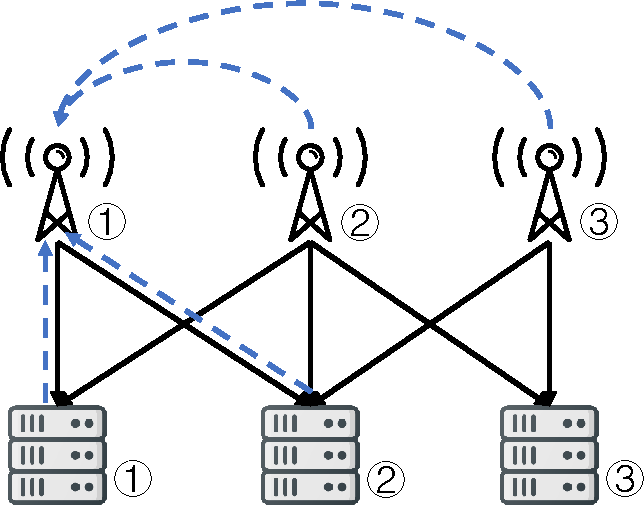
\includegraphics[width=0.60\textwidth]{osi-example.pdf}
            \caption{An Example of System Model.}
            \label{fig:osi_example}
        \end{figure*}
        Here we use a simple example below to demonstrate the impact of GSI.
        In Fig.\ref{fig:osi_example}, there are three APs and three edge servers in the edge computing system, where the solid directed lines show all the possible job dispatching paths for the APs.
        For the $1$-st AP, the OSI includes the state information of the APs indexed with $2,3$ and the edge servers indexed with $1,2$.
        The  state information of the $3$-rd edge server is out of its scope.
        {Moreover, the $3$-rd OSI includes the state information of the APs indexed with $1,2$ and the edge servers indexed with $2,3$.}
        Note that the prediction of future state distribution is essential for solving an MDP problem.
        Without GSI, it is impossible to predict the future dispatching decisions of the $3$-rd AP from the perspective of the $1$-st AP, since they observe different OSIs.
        It is thereby impossible for the $1$-st AP to predict the future state distributions of the $2$-nd edge server, lack of the dispatching decisions of the $3$-rd AP.
        As a result, the evaluation of optimal value function of the Bellman's equation if infeasible at both $1$-st and $3$-rd APs, and the distributed policy optimization for them is POMDP.
        On the other hand, if the GSI were available at all the APs without latency, there would exist global optimal scheduling policy for the MDP formulation, which should be superior to the policy proposed in our work. However, this scenario might be impractical.
        We have added the above discussion into the revised manuscript.
        % \delete{v3}{
        %     Therefore, it seems sufficient for the $1$-st AP to predict the future system states with OSI, as its dispatching decisions have no impacts on the other states (i.e., the state of the $3$-rd edge server).
        %     However, as the state information of the $3$-rd edge server is in the OSI of the $1$-st and $2$-nd AP, the changes of dispatching decisions of those APs will have \emph{indirect impacts} on the future OSI of the $1$-st AP.
        %     Therefore, the $1$-st AP should use GSI to predict the whole system states and also the global dispatching decisions to be updated on all APs.
        %     % 3. GSI is better but not scalable
        %     As GSI is not available on each AP in practice and the solution to global prediction problem is non-scalable for the scenario with massive APs and edge servers, our proposed framework prefers to use OSI instead of GSI to allow parallel dispatching decisions update by leveraging an \emph{alternative policy iteration algorithm}.
        %     To conclude, the information in GSI except OSI is useful and has \emph{indirect impacts} on the update of dispatching decisions.
        %     Hence, we cannot say the AP could observe ``global information'' with only OSI.
        % }
        % With the GSI available on each AP, the update of dispatching actions could be simultaneously carried out on each AP.
        % Therefore, the computation complexity at each AP scales linearly with respect to the size of it candidate edge server set and the algorithm can be deployed in a scenario with massive APs and edge servers.
    }

    \comments{
        \textbf{Comment 2:} Does the proposed job dispatching framework consider the possibility of packet drop? For example, in Fig. 2, What if the information broadcast by the 2-nd AP is not received by the 1-st AP?
    }
    \response{
        \textbf{Response R2-2:} \thankyou.
        % The job dispatching framework could support possibility of packet drop, a.k.a. failed transmission of system state information.
        As explained in \textbf{Response R1-1}, if packet drop occurs in the transmission of OSI, retransmissions can be requested by the receiving AP.
        Hence, the packet drop can be transferred to receiving latency of OSI, which has been addressed by the proposed algorithm.
        % with a simple retransmission schema, the $1$-st AP will request a retransmission of the broadcast information from the $2$-nd AP until success.
        We have appended a remark in Section III to address this issue in the revised manuscript.
    }

    \comments{
        \textbf{Comment 3:} In Section VI, the authors mentioned ``the distributions of job arrival, uploading latency and computation time, which are usually unknown in practice''. However, the proposed reinforcement learning approach can estimate these values in reality. What are the challenges of Algorithm 2 not being able to estimate these values?
    }
    \response{
        \textbf{Response R2-3:} \thankyou.
        We are sorry for the misunderstanding.
        Because the network may not be stationary for a long time, it is difficult to predict the distributions of job arrival, uploading latency and computation time offline in advance.
        Our proposed algorithm provides an efficient method to track these statistics in an online manner.
        We have revised the sentence to avoid misunderstanding.
        % With the help of the proposed reinforcement learning algorithm, the unknown statistics (i.e., the distributions of job arrival, uploading latency and computation time) could be learned efficiently, and then the calculation of approximate value function $W_{\Policy}(\Stat)$ is feasible.
    }

    %NOTE: normal issue
    \comments{
        \textbf{Comment 4:} The proposed MDP policy is compared with three kinds of baselines. Are there any state-of-the-art methods proposed recently?
    }
    \response{
        \textbf{Response R2-4:} \thankyou.
        %% no other works consider partial and outdated information
        In fact, the three heuristic baseline schemes are efficient and widely used as performance baselines in the existing literature with many different scenarios \cite{tan-online, IOTJ19-CaoJ, JSAC17-LyuX, TMC19-JosiloS}.
        However, there is no state-of-the-art job dispatching design for our considered scenario.
        As mentioned in the introduction section of the original manuscript, ``most existing works assume a centralized job dispatcher, which has timely and complete knowledge of the global system status \cite{tan-online,IOTJ18-FanQ,mdp-globecom,mdp-tvt,MASS18-MengZ,latency-EDGE19,MOBIHOC19-ZhouZ,TOC19-LiuC,JSAC19-AlameddineHA}.''
        To the best of our knowledge, there are no existing methods proposed to solve job dispatching with \textbf{outdated and partial information} of the system, not to mention the cooperation of multiple dispatchers in the system.
        %
        % and distributes the dispatching decisions to all the APs without delay .
        %% our baselines are heuristic but efficient
        % Hence, we use three heuristic but efficient baselines in the original manuscript to profile the performance of the proposed solution framework \algname. %under different parameter settings
        % Specifically, 
        % \emph{Random Policy} randomly dispatches the jobs for load balancing,
        % \emph{Selfish Policy} chooses the edge server with minimum time only awareness of statistical parameters (expected uploading time and processing time) but regardless of queueing status,
        % and \emph{Queue-aware Policy} chooses the edge server awareness of queueing status of the edge servers but with outdated observation. % is invariant of \brlatency
        %% why MDP works (extended answer)
        % Moreover, compared to other works leveraging MDP in scheduling algorithm design for edge computing systems \cite{mdp-jcin,mdp-globecom,mdp-tvt}, our proposed policy could solve Bellman's equation efficiently in the considered scenario.
        % There are only two works consider outdated information by leveraging Lyapunov optimization to achieve queue stability, because it is infeasible to solve the optimization of queue length in the considered scenario.
        % the existence of \brlatency~may not raise a significant challenge to the algorithm design with Lyapunov optimization.
        % In fact, the design of distributed dispatchers with \brlatency~could be more challenging.
        % For example, the signaling latencies at distributed dispatchers could be different, and the synchronization of their dispatching decisions becomes infeasible.

        % \wangr{
        %     As mentioned in the introduction section of the original manuscript, MDP has already been applied in scheduling algorithm design for edge computing systems \cite{mdp-jcin,mdp-globecom,mdp-tvt}.
        %     However, to the best of our knowledge, there are no existing methods proposed to solve job dispatching with outdated and partial information of the system.
        %     Because it is infeasible to solve Bellman's equation in the considered scenario.
        %     In fact, the three baselines are commonly considered in the existing literature.
        %     For example, \dots
        % }
    }

    \comments{
        \textbf{Comment 5:} It is recommended to enlarge the legends of Figures 5 and 7.
    }
    \response{
        \textbf{Response R2-5:} \thankyou.
        We have enlarged the legends of Figures 5 and 7.
    }
    %-------------------------------- Response to Reviewer 2 -------------------------------%


    \bibliographystyle{IEEEtran}
    \bibliography{extra.bib}
\end{document}